\section{Methodology}

\subsection{Intel Image Dataset}

The Intel Image Classification Dataset \cite{intel_image_classification_kaggle} was curated
as part of a data hackathon organized
by Intel\footnote{https://www.intel.com/content/www/us/en/homepage.html}
on the online platform Kaggle\footnote{https://www.kaggle.com/},
with the aim of fostering engagement and innovation within data science communities.
The dataset comprises 25,000 RGB color images,
each with a resolution of 150 $\times$ 150 pixels,
depicting a variety of natural and urban scenes from around the world.
The images, originally captured by Jan Böttinger
on Unsplash\footnote{https://unsplash.com/},
are labeled into six distinct classes: buildings, forest, glacier, mountain, sea, and street.

The dataset is partitioned into three subsets: approximately 14,000 images for training,
3,000 images for testing, and 7,000 images for prediction tasks.
Each subset is provided as a separate zipped file on Kaggle.

The primary objective of this dataset is to support participants
in developing and evaluating image classification models.
By providing a diverse and well-labeled collection of scenes,
the dataset encourages the development of robust classification algorithms
capable of distinguishing objects in various environments with reasonable accuracy.

\subsection{Model Architecture}
\label{sec:method:model_architecture}

\begin{figure}[ht]
    \centering
    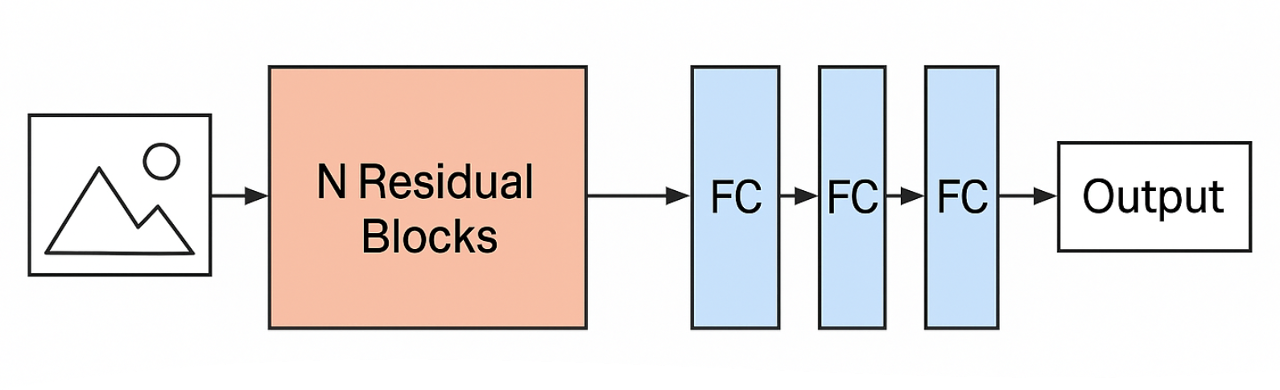
\includegraphics[width=0.5\textwidth]{assets/model-architecture.png}
    \caption{Custom CNN model Architecture}
    \label{fig:model_architecture}
\end{figure}

In this section, we describe the architecture of the teacher model.
We implemented a custom \gls*{cnn} model, incorporating residual blocks \cite{he2016deep},
which hierarchically extract and aggregate spatial features from the input images
before mapping them to one of six scene categories.

The model consists of 12 residual blocks,
progressively increasing the channel capacity while reducing the spatial resolution,
and a fully connected classifier that sequentially reduces feature dimensions through 1024, 512, 256, 64, and finally 6 outputs.
In total, the model contains 26,534,358 parameters.

All operations in the model are performed using 32-bit floating point precision,
which is the default in PyTorch \cite{paszke2019pytorch}
for most GPUs.

\subsection{Weight Reduction}
\label{sec:method:weight_reduction}

To create lighter student models from the teacher architecture,
we reduced both the number of residual blocks and the depth of the classifier.
Four reduced models were created, excluding the teacher model,
with 10, 8, 6, and 4 residual blocks, respectively,
and classifier configurations of (512, 256, 64, 16), (256, 64, 16), (128, 64, 16), and (64, 32) layers.
The number of parameters in these models are 6,601,686, 1,648,470, 408,854, and 98,294, respectively.

\subsection{Precision Quantization}
\label{sec:method:precision_quantization}

Quantization was applied to both model weights and floating point operations
to further reduce computational cost.
Two different levels of precision were explored: 16-bit and 8-bit floating point.
To implement quantization,
we used \texttt{torch.set\_default\_dtype()} along with the \texttt{bitsandbytes}~\cite{bitsandbytes} Python framework.
